\documentclass{article}
\usepackage{graphicx}  
\usepackage[landscape]{geometry}
\usepackage[pdftex]{color}
\usepackage{url}
\usepackage{multicol}
\usepackage{amsmath}
\usepackage{amsfonts}
\newcommand{\ex}{\color{blue}}
\pagestyle{empty}
\newcommand{\kr}[2]{\left(\frac{#1}{#2}\right)}
\advance\topmargin-.9in
\advance\textheight2in
\advance\textwidth3.0in
\advance\oddsidemargin-1.45in
\advance\evensidemargin-1.45in
\parindent0pt
\parskip2pt
\newcommand{\hr}{\centerline{\rule{3.5in}{1pt}}}
\newcommand{\ZZ}{\mathbf{Z}}
\begin{document}
\begin{multicols*}{3}
\begin{center}
\textbf{Sage Quick Reference:\\Elementary Number Theory}\\
William Stein\\
Sage Version 3.4\\
\url{http://wiki.sagemath.org/quickref}\\
GNU Free Document License, extend for your own use\\
\end{center}
\vspace{-2ex}

 \hr
Everywhere $m,n,a,b, etc.$ are elements of \texttt{ZZ}\\
\verb|          ZZ = | $\mathbf{Z} = $ all integers\\
\vspace{-3ex}

%*********************************************
 \hr\textbf{Integers}
\vspace{-2ex}
$$\ldots, -2, -1, 0, 1, 2, 3, 4, 5, 6, 7, 8, 9, 10, \ldots$$
\vspace{-5ex}

$n$ divided by $m$ has {\em remainder} \texttt{n \% m}

\texttt{gcd(n,m), gcd({\it list})}

extended gcd $g = sa + tb=\gcd(a,b)$: \texttt{g,s,t=xgcd(a,b)}

\texttt{lcm(n,m), lcm({\it list})}

binomial coefficient $\binom{m}{n} = $ \texttt{binomial(m,n)}

digits in a given base: \texttt{n.digits({\it base})}

number of digits: \texttt{n.ndigits({\it base})}

({\it base} is optional and defaults to 10)

divides $n\mid m$: \texttt{n.divides(m)} if $nk=m$ some $k$

divisors -- all $d$ with $d\mid n$: \texttt{n.divisors()}

factorial -- $n! = $ \texttt{n.factorial()}


%*********************************************
 \hr\textbf{Prime Numbers}
\vspace{-2ex}

$$2, 3, 5, 7, 11, 13, 17, 19, 23, 29, 31, 37, 41, 43, 47, \ldots$$
\vspace{-4ex}

factorization: \texttt{factor(n)}

primality testing: \texttt{is\_prime(n)}, \texttt{is\_pseudoprime(n)}

prime power testing: \texttt{is\_prime\_power(n)}

$\pi(x) = \#\{p: p \leq x\text{ is prime}\} = $ \texttt{prime\_pi(x)}

set of prime numbers: \texttt{Primes()}

$\{p : m \leq p < n\text{ and $p$ prime}\} = $\texttt{prime\_range(m,n)}

prime powers: \texttt{prime\_powers(m,n)} 

first $n$ primes: \texttt{primes\_first\_n(n)}

next and previous primes: \texttt{next\_prime(n)}, \\
\mbox{}\quad\texttt{previous\_prime(n)},  \texttt{next\_probable\_prime(n)}

prime powers:\\
\mbox{}\quad\texttt{next\_prime\_power(n)}, \texttt{pevious\_prime\_power(n)}


Lucas-Lehmer test for primality of $2^p-1$\\
\verb|  def is_prime_lucas_lehmer(p):|\\
\verb|      s = Mod(4, 2^p - 1)|\\
\verb|      for i in range(3, p+1): s = s^2 - 2|\\
\verb|      return s == 0|\\



%*********************************************
 \hr\textbf{Modular Arithmetic and Congruences}

{\tiny
\verb|k=12; m = matrix(ZZ, k, [(i*j)%k for i in [0..k-1] for j in [0..k-1]]); m.plot(cmap='gray')|}

\mbox{}\qquad\qquad
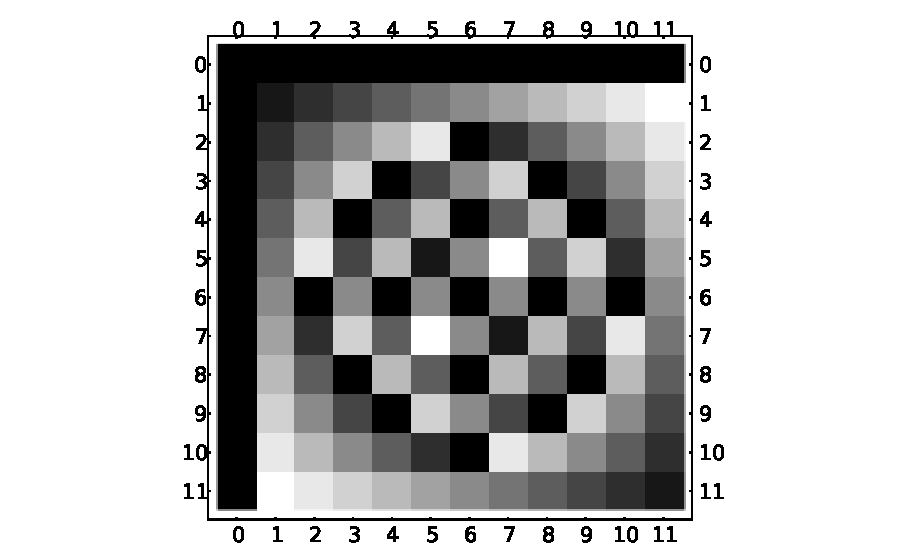
\includegraphics[width=14em]{mod12}

Euler's $\phi(n)$ function: \texttt{euler\_phi(n)}

Kronecker symbol $\kr{a}{b} = $ \texttt{kronecker\_symbol(a,b)}

Quadratic residues: \texttt{quadratic\_residues(n)}

Quadratic non-residues: \texttt{quadratic\_residues(n)}

ring $\ZZ/n\ZZ = $ \texttt{Zmod(n) = IntegerModRing(n)}

$a$ modulo $n$ as element of $\ZZ/n\ZZ$: \texttt{Mod(a, n)}


primitive root modulo $n = $ \texttt{primitive\_root(n)}

inverse of $n\pmod{m}$: \texttt{n.inverse\_mod(m)}

power $a^n\pmod{m}$: \texttt{power\_mod(a, n, m)}

Chinese remainder theorem: \texttt{x = crt(a,b,m,n)}\\
\mbox{} \qquad finds $x$ with $x\equiv a\pmod{m}$ and $x\equiv b\pmod{n}$

discrete log: \texttt{log(Mod(6,7), Mod(3,7))}

order of $a\pmod{n}=$\texttt{Mod(a,n).multiplicative\_order()}

square root of $a\pmod{n}=$\texttt{Mod(a,n).sqrt()}

%*********************************************
 \hr\textbf{Special Functions}

{\tiny\verb|complex_plot(zeta, (-30,5), (-8,8))|}

\mbox{}\qquad\qquad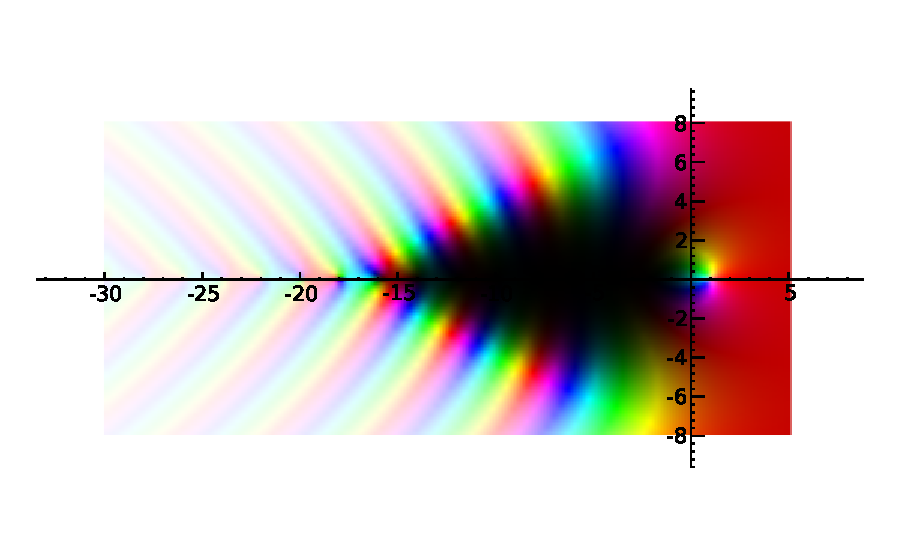
\includegraphics[width=15em]{zeta}

$\zeta(s) = \prod_{p} \frac{1}{1-p^{-s}} = \sum \frac{1}{n^s} = $ \texttt{zeta(s)}

$\text{Li}(x) = \int_{2}^{x} \frac{1}{\log(t)} dt = $ \texttt{Li(x)}

$\Gamma(s) = \int_0^{\infty} t^{s-1}e^{-t}dt = $ \texttt{gamma(s)}

\mbox{}
\vspace{9em}

%*********************************************
 \hr\textbf{Continued Fractions}

{\tiny \verb|continued_fraction(pi)|}

{\small $$
\pi = 3+ \frac{\displaystyle 1}{\displaystyle 7+ \frac{\displaystyle 1}{\displaystyle 15+ \frac{\displaystyle 1}{\displaystyle 1+ \frac{\displaystyle 1}{\displaystyle 292 + \cdots}}}}$$}

continued fraction: \texttt{c=continued\_fraction(x, {\it bits})}

convergents: \texttt{c.convergents()}

convergent numerator $p_n =$ \texttt{c.pn(n)}

convergent denominator $q_n =$ \texttt{c.qn(n)}

value: \texttt{c.value()}

 
%*********************************************
 \hr\textbf{Elliptic Curves}

{\tiny
\verb|EllipticCurve([0,0,1,-1,0]).plot(plot_points=300,thickness=3)|}

\mbox{}\qquad\qquad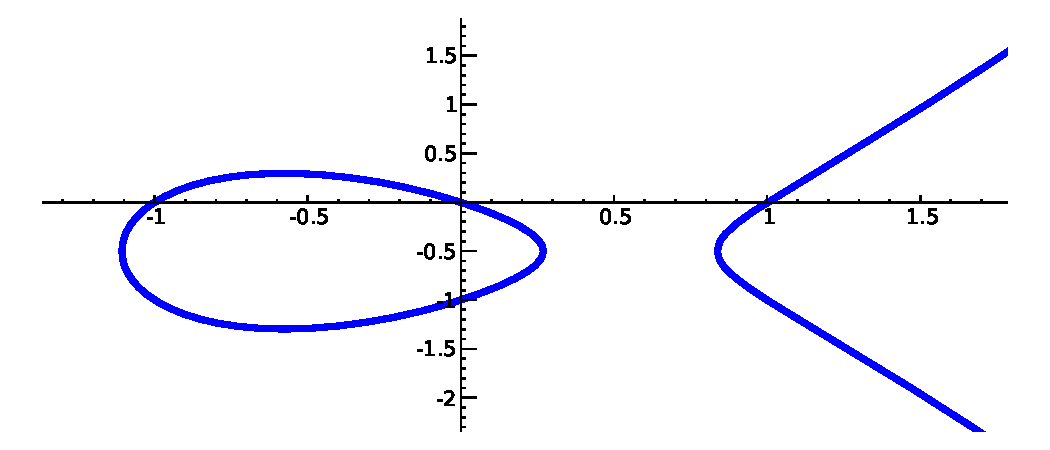
\includegraphics[width=10em]{ec}

\mbox{}\quad\texttt{E = EllipticCurve([$a_1,a_2,a_3,a_4,a_6$])}
\vspace{-2ex}

$$y^2 + a_1 xy + a_3 y = x^3 + a_2 x^2 + a_4 x + a_6$$

conductor $N$ of $E = $\texttt{E.conductor()}

discriminant $\Delta$ of $E = $\texttt{E.discriminant()}

rank of $E =$  \texttt{E.rank()}

free generators for $E(\mathbf{Q}) = $ \texttt{E.gens()}

$j$-invariant $=$ \texttt{E.j\_invariant()}

$N_p = \#\{\text{solutions to $E$ modulo $p$}\} = $ \texttt{E.Np({\it prime})}

$a_p = p+1 - N_p = $\texttt{E.ap({\it prime})}

$L(E,s) = \sum \frac{a_n}{n^s} = $ \texttt{E.lseries()}

$\text{ord}_{s=1}L(E,s) = $ \texttt{E.analytic\_rank()}


%*********************************************
 \hr\textbf{Elliptic Curves Modulo $p$}

{\tiny
\verb|EllipticCurve(GF(997), [0,0,1,-1,0]).plot()|}

\mbox{}\qquad\qquad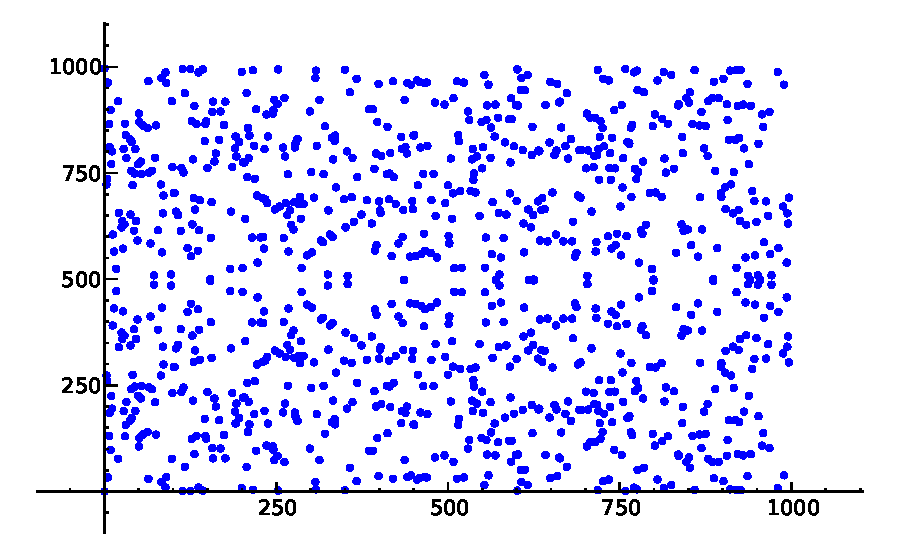
\includegraphics[width=7em]{ecmodp}

\mbox{}\quad\texttt{E = EllipticCurve(GF(p), [$a_1,a_2,a_3,a_4,a_6$])}

$\#E(\mathbf{F}_p) = $ \texttt{E.cardinality()}

generators for $E(\mathbf{F}_p) = $ \texttt{E.gens()}

$E(\mathbf{F}_p) = $\texttt{E.points()}










%%*********************************************
% \hr\textbf{Binary Quadratic Forms}
%\texttt{QuadraticForm}

%*********************************************
% \hr\textbf{Quadratic Fields}
%\texttt{ZZ[I]}
%\texttt{QuadraticField}

%*********************************************
% \hr\textbf{Cyclotomic Fields}
%\texttt{CyclotomicField}
%\texttt{Gauss sums}


%*********************************************
% \hr\textbf{Finite Fields}
%\texttt{GF(q)}



\end{multicols*}

\end{document}
